\documentclass[../main.tex]{subfiles}
\begin{document}
\chapter{Rigid Bodies}
Rigid body problems are a class of $N$-body problems where distances between the $N$ particles are fixed:
\[
  |\vec{x}_i - \vec{x}_j| = \text{constant}
\]
These are often tractable problems and usually arise due to very strong internal forces between particles.
Such a system of particles is known as a \textit{rigid body}.

The only motions a rigid body can experience are \textbf{translations of the centre of mass}, which we covered in \cref{systemsOfParticles}, and \textbf{rotations}, which we will cover now.
\section{Rotations}
\label{rigidRotations}
\subsection{Angular Velocity}
In three dimensions, rotations are described by a vector quantity $\vec{\omega}$ called the \textit{angular velocity}.
\begin{definition}[Angular Velocity]
  The \textit{angular velocity} $\vec{\omega}$ is defined as:
  \[
    \vec{\omega} = \omega \uvec{n}
  \]
  where $\uvec{n}$ points along the axis of rotation and $\omega = |\vec{\omega}| = |\dot{\theta}|$ is the angular speed of rotation.
\end{definition}
\begin{remark}[Right Hand Rule]
  We define $\uvec{n}$ so that it always points in the direction where if you align you right hand thumb along the positive direction of the axis of rotation, the rotation is in the direction that your fingers curl.
\end{remark}
The key equation for rotations is:
\begin{equation}
  \dot{\vec{x}} = \vec{\omega} \times \vec{x} \label{angularVelocityCross}
\end{equation}
This can be seen in the following diagram:
\begin{center}
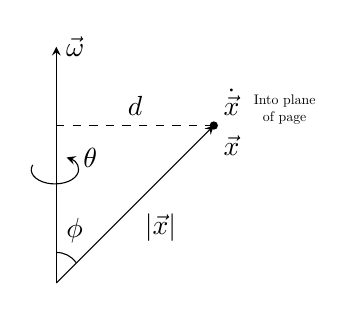
\begin{tikzpicture}[>=stealth]
  \draw[->] (0, 0)  -- (0, 3) node[right] {$\vec{\omega}$};
  \draw[->] (0, 0) -- (2, 2) node[below right] {$\vec{x}$} node[midway, below right] {$|\vec{x}|$};
  \fill (2, 2) circle (1.5pt) node[above right] {$\dot{\vec{x}}$};
  \node[text width=2cm, align=center, scale=0.5] at (2.9, 2.2) {Into plane of page};
  \draw[dashed] (2, 2) -- (0, 2) node[midway, above] {$d$};
  \draw[->, yscale=0.6] (-0.3,2.5) arc [start angle=-200,end angle=60,radius=0.3] node[xshift=0.3cm] {$\theta$};
  \draw (0.25,0.26) arc [start angle=35,end angle=90,radius=0.3] node[above right] {$\phi$};
\end{tikzpicture}
\end{center}
$\dot{\vec{x}}$ is orthogonal to both $\vec{\omega}$ and $\vec{x}$ and acts \textbf{into the plane of the page} in the above diagram.

The magnitude of $\uvec{n} \times \vec{x}$ is the distance between $\vec{x}$ and the axis of rotation:
\[
  |\uvec{n} \times \vec{x}| = |\uvec{n}||\vec{x}|\sin \phi = d
\]
and so:
\[
  |\dot{\vec{x}}| = \omega|\uvec{n} \times \vec{x}| = \omega d
\]
Therefore, the particle has speed $\omega d$, so $|\dot{\theta}| = \omega$

In addition to the angular velocity, a rotation must also specify a point about which the axis of rotation passes through.
For example, if we specify that the axis of rotation is the $z$-axis, then this does \textbf{not} specify the rotation as we do not know where the object is relative to this axis.
In the diagram, the vector $\vec{x}$ is measured from a point on the axis and we could have taken any point on the axis and it would be the same rotation.
The upshot of this is that in \cref{angularVelocityCross}, $\vec{x}$ must be relative to some arbitrary point on the axis of rotation.
\subsection{Moment of Inertia}
A particle rotating with angular velocity $\vec{\omega}$ has kinetic energy:
\begin{align*}
  T &= \frac{1}{2} m\dot{\vec{x}} \cdot \dot{\vec{x}} \\
    &= \frac{1}{2} m(\vec{\omega} \times \vec{x}) \cdot (\vec{\omega} \times \vec{x}) \\
    &= \frac{1}{2} m \omega^2 (\uvec{n} \times \vec{x}) \cdot (\uvec{n} \times \vec{x}) \\
    &= \frac{1}{2} m \omega^2 d^2
\end{align*}
where $d = |\uvec{n} \times \vec{x}|$ the perpendicular distance of $\vec{x}$ to the axis of rotation.

In a rigid body, all particles rotate with the same angular velocity $\vec{\omega}$, i.e.:
\[
  \dot{\vec{x}}_i = \vec{\omega} \times \vec{x}_i
\]
This ensures that the distances between particles remain fixed:
\begin{align*}
  \deriv{}{t}|\vec{x}_i - \vec{x}_j|^2 &= 2(\dot{\vec{x}}_i - \dot{\vec{x}}_j) \cdot (\vec{x}_i - \vec{x}_j) \\
                                       &= 2 [\vec{\omega} \times (\vec{x}_i - \vec{x}_j)] \cdot (\vec{x}_i - \vec{x}_j) \\
                                       &= 0
\end{align*}
and so $|\vec{x}_i - \vec{x}_j|$ is constant for all pairs of particles $i, j$ and so it remains a rigid body.
\begin{definition}[Moment of Inertia]
  For a particular choice of axis, the \textit{moment of inertia} $I$, of a rigid body is:
  \[
    I = \sum_{i = 1}^{N} m_i d^2_i
  \]
  where $d_i$ is the perpendicular distance of the $i$-th particle from the axis of rotation.
\end{definition}
The total kinetic energy of a rigid body is then:
\begin{align}
  T &= \frac{1}{2} \sum_{i = 1}^{N} m_i \dot{\vec{x}}_i \cdot \dot{\vec{x}}_i \nonumber \\
    &= \frac{1}{2} \omega^2 \sum_{i = 1}^{N} m_i d^2_i \nonumber \\
    &= \frac{1}{2} I \omega^2 \label{totalRotationalKE}
\end{align}
\begin{remark}
  We see that $I$ is like the ``rotational mass'', the larger it is, the harder it is to rotate the rigid body.
\end{remark}

In a rigid body, the angular momentum is:
\begin{align*}
  \vec{L} &= \sum_{i = 1}^{N} m_i \vec{x}_i \times \dot{\vec{x}}_i \\
          &= \sum_{i = 1}^{N} m_i \vec{x}_i \times (\vec{\omega} \times \vec{x}_i)
\end{align*}
In this course, we will only consider the component of $\vec{L}$ along the axis of rotation $\uvec{n}$, i.e. $L = \vec{L} \cdot \uvec{n}$ so:
\begin{align*}
  L &= \omega \left(\sum_{i = 1}^{N} m_i \vec{x}_i \times (\uvec{n} \times \vec{x}_i)\right) \cdot \uvec{n} \\
    &= \omega \sum_{i = 1}^{N} m_i (\vec{x}_i \times (\uvec{n} \times \vec{x}_i)) \cdot \uvec{n} \\
    &= \omega \sum_{i = 1}^{N} m_i (\uvec{n} \times \vec{x}_i) \cdot (\uvec{n} \times \vec{x}_i) \text{ as $(\vec{a} \times \vec{b}) \cdot \vec{c} = (\vec{c} \times \vec{a}) \cdot \vec{b}$} \\
    &= \omega \sum_{i = 1}^{N} m_i d^2_i \\
    &= \omega I
\end{align*}
\begin{remark}
  Linear momentum is velocity times mass and here angular momentum along the axis is angular velocity times moment of inertia, so again in the moment of inertia acts like a ``rotational mass''.
\end{remark}
Recall from \cref{totalAngularMomentum}, that external the \textit{torque} $\vec{G}$ changes angular momentum, that is, $\dot{\vec{L}} = \vec{G}$.
If the torque is along the axis of rotation, then $\vec{G} = G\uvec{n}$ for some scalar $G$.
If we dot both sides of $\dot{\vec{L}} = \vec{G}$  to compare components along the axis, we have:
\begin{equation}
  \dot{\vec{L}} \cdot \uvec{n} = \vec{G} \cdot \uvec{n} \implies \dot{L} = G \implies \dot{\omega}I = \ddot{\theta}I = G \label{torqueMomentOfInertia}
\end{equation}
\begin{remark}[Note]
  So far, all of this depends on the axis of rotation that we choose and is not an intrinsic property of the body.

  In Part II, we will define a more invariant \textit{inertia tensor} that packages up all the information needed to find the moment of inertia of a rigid body about \textbf{any axis}.
\end{remark}
\subsection{Computing Moment of Inertia}
\subsubsection{Approximating Sums with Integrals}
The calculate the moment of inertia, we can utilise that for large $N$, the particles are densely spaced and so we can approximate the unwieldy sums using integrals.

For any function $f(\vec{x})$:
\[
  \sum_{i = 1}^{N} m_i f(\vec{x}_i) \approx \int \rho(\vec{x}) f(\vec{x}) \d^3{\vec{x}}
\]
where $\rho$ is the \textit{density} of the rigid body at $\vec{x}$, although we typically consider situations with uniform density, i.e. $\rho(\vec{x}) = \rho_0\ \forall x \in \R^3$.

If we want the mass of the body $M$, we set $f(\vec{x}) = 1$ and so:
\[
  M = \int \rho(\vec{x}) \d^3{\vec{x}}
\]
Similarly, for the moment of inertia, we set $f(\vec{x}) = x^2_{\perp}$ where $x_{\perp}$ is the perpendicular distance of $\vec{x}$ from the axis of rotation, and so:
\[
  I = \int \rho(\vec{x}) x^2_\perp \d^3{\vec{x}}
\]
\begin{example}[Moments of Inertia for Basic Shapes]
  \label{basicInertia}
  Consider the following rigid bodies with a constant density $\rho$.
  \begin{enumerate}
    \item Consider a 1D ring $R$ of radius $a$:
      \begin{center}
      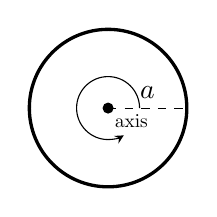
\begin{tikzpicture}[>=stealth]
        \draw[very thick] (0, 0) circle (1);
        \draw[dashed] (0, 0) -- (1, 0) node[midway, above] {$a$};
        \fill (0, 0) circle (2pt) node[below right, scale=0.7] {axis};
        \draw[->] (0.4, 0) arc [start angle=0,end angle=300,radius=0.4];
      \end{tikzpicture}
      \end{center}
      Its mass is:
      \[
        M = 2\pi a \rho
      \]
      and if it is rotating through its centre the moment of inertia is:
      \[
        I = \int_{R} \rho a^2 \d{\vec{x}} = 2\pi \rho a^3
      \]
      as the length of $R$ is $2 \pi a$.
      We can then relate the two by $I = Ma^2$.
    \item Consider a 1D rod of length $\ell$:
      \begin{center}
      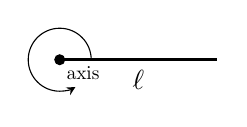
\begin{tikzpicture}[>=stealth]
        \draw[very thick] (0, 0) -- (2, 0) node[midway, below] {$\ell$};
        \fill (0, 0) circle (2pt) node[below right, scale=0.7] {axis};
        \draw[->] (0.4, 0) arc [start angle=0,end angle=300,radius=0.4];
      \end{tikzpicture}
      \end{center}
      Its mass is:
      \[
        M = \ell \rho
      \]
      and if it is rotating about one of its ends, the moment of inertia is:
      \[
        I = \rho \int_{0}^{\ell} x^2 \d{x} = \frac{\rho \ell^3}{3} = \frac{1}{3}M\ell^2
      \]
    \item Consider a 2D disc $D$ of radius $a$:
      \begin{center}
      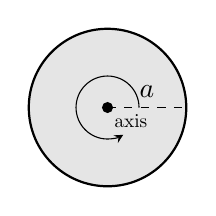
\begin{tikzpicture}[>=stealth]
        \filldraw[fill=gray!20, draw=black, thick] (0, 0) circle (1);
        \draw[dashed] (0, 0) -- (1, 0) node[midway, above] {$a$};
        \fill (0, 0) circle (2pt) node[below right, scale=0.7] {axis};
        \draw[->] (0.4, 0) arc [start angle=0,end angle=300,radius=0.4];
      \end{tikzpicture}
      \end{center}
      Its mass is:
      \[
        M = \pi a^2 \rho
      \]
      and if it is rotating through its centre, the moment of inertia is:
      \[
        I = \int_{D} \rho x^2_\perp \d^2{\vec{x}}
      \]
      Using methods from Vector Calculus, we change to plane polar coordinates on the disc.
      We have $x_{\perp} = r$ and we introduce the Jacobian $|J| = r$ so:
      \begin{align*}
        I &= \int_{0}^{2\pi} \int_{0}^{a} \rho r^2 \cdot r\d{r} \d{\theta} \\
          &= \rho \int_{0}^{2\pi} \d{\pi} \int_{0}^{a} r^3 \d{r} \\
          &= \frac{\pi}{2}\rho a^4 = \frac{1}{2}Ma^2
      \end{align*}
    \item For a 3D sphere $V$ of radius $a$, its mass is $M = \frac{4}{3} \pi a^3 \rho$ and if it is rotating about an axis through its centre, the moment of inertia is:
      \[
        I = \int_{V} \rho x^2_\perp \d^3{\vec{x}}
      \]
      Using methods from Vector Calculus, we change to spherical coordinates using the axis of rotation as the $z$-axis.
      We have $x_{\perp} = r \sin \theta$ and we introduce the Jacobian $|J| = r^2 \sin \theta$ so:
      \begin{align*}
        I &= \int_{0}^{2\pi} \int_{0}^{\pi} \int_{0}^{a} \rho(r \sin \theta)^2 \cdot r^2 \sin \theta \d{r} \d{\theta} \d{\phi} \\
          &= \rho\int_{0}^{2\pi} \d{\phi} \int_{0}^{\pi} \sin^3 \theta \d{\theta} \int_{0}^{a} r^4 \d{r} \\
          &= \rho \cdot 2 \pi \cdot \frac{4}{3} \cdot \frac{a^5}{5} \\
          &= \frac{8\pi}{15} \rho a^5 = \frac{2}{5}Ma^2
      \end{align*}
  \end{enumerate}
\end{example}
\begin{remark}
  In these examples, we see that if the shape of the rigid body is defined by a single length $a$, then $I = kMa^2$ where $k$ is some constant.
\end{remark}
\subsubsection{Perpendicular Axis Theorem}
\begin{lemma}[Perpendicular Axis Theorem]
  For a 2D rigid body, sometimes called a \textit{lamina}, on the $(x, y)$-plane, its moments of inertia $I_x$, $I_y$, and $I_z$ about the $x$, $y$ and $z$ axes respectively are:
  \begin{align*}
    I_x &= \int \rho(\vec{x}) \cdot y^2 \d^2{\vec{x}} \\
    I_y &= \int \rho(\vec{x}) \cdot x^2 \d^2{\vec{x}} \\
    I_z &= \int \rho(\vec{x}) \cdot (x^2 + y^2) \d^2{\vec{x}} = I_x + I_y
  \end{align*}
\end{lemma}
\begin{proof}
  If we take the $x$-axis to be the axis of rotation, then the perpendicular distance of a particle at $(x, y)$ to the axis is just $y$ and so:
  \[
    I_x = \int \rho(\vec{x}) \cdot y^2 \d^2{\vec{x}}
  \]
  and similarly about the $y$ axis.

  If we take the $z$-axis to be the axis of rotation, then the perpendicular distance of a particle at $(x, y)$ to the axis is just its distance from the origin and so:
  \[
    I_z = \int \rho(\vec{x}) \cdot \left(\sqrt{x^2 + y^2}\right)^2 \d^2{\vec{x}} = \int \rho(\vec{x}) \cdot (x^2 + y^2) \d^3{\vec{x}} = I_x + I_y
  \]
\end{proof}
\subsubsection{Parallel Axis Theorem}
\begin{lemma}[Parallel Axis Theorem]
  If we know the moment of inertia of a 3D rigid body about some axis through the CoM, then the moment of inertia $I_{\text{para}}$ about any other axis parallel to that axis is given by:
  \label{parallelAxisTheorem}
  \[
    I_{\text{para}} = I_{\text{CoM}} + Mh^2
  \]
  where $h$ is the distance between the two axes.
\end{lemma}
\begin{remark}
  Since $h^2 \geq 0$, $I_{\text{para}} \geq I_{\text{CoM}}$.
  This means that the moment of inertia for a given axis direction is minimised when the axis passes through the CoM.
\end{remark}
\begin{proof}
  Recall from \cref{relativeSum}, that if we write $\vec{x}_i = \vec{R} + \vec{y}_i$, then:
  \[
    \sum_{i = 1}^{N} m_i \vec{y}_i = \vec{0}
  \]
  Here we have chosen the origin to be \textbf{on the parallel axis} as we are finding the moment of inertia about this axis.

  The moment of inertia is:
  \begin{align*}
    I_{\text{para}} &= \sum_{i = 1}^{N} m_i (\uvec{n} \times \vec{x}_i) \cdot (\uvec{n} \times \vec{x}_i) \\
                    &= \sum_{i = 1}^{N} m_i (\uvec{n} \times [\vec{R} + \vec{y}_i]) \cdot (\uvec{n} \times [\vec{R} + \vec{y}_i]) \\
                    &= \sum_{i = 1}^{N} m_i [(\uvec{n} \times \vec{R}) \cdot (\uvec{n} \times \vec{R}) + (\uvec{n} \times \vec{y}_i) \cdot (\uvec{n} \times \vec{y}_i) + 2(\uvec{n} \times \vec{R}) \cdot (\uvec{n} \times \vec{y}_i)] \\
                    &= \sum_{i = 1}^{N} m_i [h^2 + (\uvec{n} \times \vec{y}_i) \cdot (\uvec{n} \times \vec{y}_i)] + 2(\uvec{n} \times \vec{R}) \cdot \left(\cancelto{\vec{0}}{\uvec{n} \times \sum_{i = 1}^{N} m_i \vec{y}_i}\right) \\
                    &= Mh^2 + \sum_{n = 1}^{N} m_i (\uvec{n} \times \vec{y}_i) \cdot (\uvec{n} \times \vec{y}_i) \\
                    &= Mh^2 + I_{\text{CoM}}
  \end{align*}
  Since $(\uvec{n} \times \vec{y}_i) \cdot (\uvec{n} \times \vec{y}_i)$ is the perpendicular distance of the $i$-th particle to the CoM axis.
\end{proof}
\begin{example}
  Revisiting the 2D disc from \cref{basicInertia} but now with the axis on the edge of the disc.
  \begin{center}
  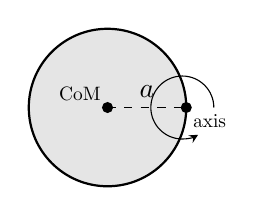
\begin{tikzpicture}[>=stealth]
    \filldraw[fill=gray!20, draw=black, thick] (0, 0) circle (1);
    \draw[dashed] (0, 0) -- (1, 0) node[midway, above] {$a$};
    \fill (1, 0) circle (2pt) node[below right, scale=0.7] {axis};
    \fill (0, 0) circle (2pt) node[above left, scale=0.7] {CoM};
    \draw[->] (1.35, 0) arc [start angle=0,end angle=300,radius=0.4];
  \end{tikzpicture}
  \end{center}
  So the moment of inertia about this parallel axis is:
  \[
    I = I_{\text{CoM}} + Ma^2 = \frac{1}{2}Ma^2 + Ma^2 = \frac{3}{2}Ma^2
  \]
  We see that it is harder to rotate the disc when the axis is positioned at the edge of the disc than when it is in the centre.
\end{example}
\section{Motion of Rigid Bodies}
\subsection{Translational Motion}
We can also allow the centre of mass to move as the body rotates so $\vec{R}$ becomes $\vec{R}(t)$.
\[
  \vec{x}_i = \vec{R}(t) + \vec{y}_i
\]
Since the particles cannot move relative to each other, the behaviour of the $\vec{y}_i$ will capture the rotation of the body about the CoM, provided $\dot{\vec{y}}_i = \vec{\omega} \times \vec{y}_i$

We can differentiate to find the velocity $\dot{\vec{x}}_i$:
\[
  \dot{\vec{x}}_i = \dot{\vec{R}} + \dot{\vec{y}}_i
\]
We saw in \cref{totalKE} that the kinetic energy can be split up as as:
\[
  T = \frac{1}{2}M|\dot{\vec{R}}|^2 + \frac{1}{2} \sum_{i = 1}^{N} m_i |\dot{\vec{y}}_i|^2
\]
Since this is a rigid body, the only allowed motion for $\vec{y}_i$ is rotation so $\dot{\vec{y}}_i = \vec{\omega} \times \vec{y}_i$.
Using \cref{totalRotationalKE} with the axis through the CoM and using the relative positions $\vec{y}_i$, we have:
\begin{equation}
  T = \underbrace{\frac{1}{2}M|\dot{\vec{R}}|}_{\text{translational}} + \underbrace{\frac{1}{2} I_{\text{CoM}} \omega^2}_{\text{rotational}} \label{rigidKESplit}
\end{equation}
So we have split the kinetic energy into translational and rotational kinetic energies.

Recall from \cref{totalEnergy} that:
\[
  V = \sum_{i = 1}^{N}  V_i(\vec{x}_i) + \sum_{i < j} V_{ij}(|\vec{x}_i -  \vec{x}_j|)
\]
Since we are working with rigid bodies, the distances between particles are fixed and so the second sum is just a constant.
This means that it will disappear when differentiated to find the force and so can be ignored.

One nice case is constant gravitational field, $V_i(\vec{x}_i) = m_i gz_i$ and so:
\begin{equation}
  V = \sum_{i = 1}^{N} V_i(\vec{x}_i) = g \sum_{i = 1}^{N} m_i z_i(t) = gMR_z(t) \label{rigidPotential}
\end{equation}
where $R_z(t)$ is the $z$-component of the CoM.
This means that the rigid body acts just like a point particle with mass $M$ at the CoM.
\begin{remark}[Note]
  Here we used an axes that passes through the CoM, however, in some cases it may be easiest to consider an axis that does not pass through the CoM.
\end{remark}
\subsection{Motion of a Pendulum}
Consider a uniform rigid rod pendulum of mass $M$ and length $L$:
\begin{center}
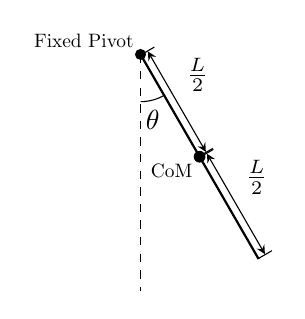
\begin{tikzpicture}[>=stealth]
  \fill (0, 0) circle (2pt) node[above left, scale=0.7] {Fixed Pivot};
  \draw[dashed]  (0, 0) -- (0, -3);
  \draw[rotate=30, thick] (0, 0) -- (0, -3) node[midway, below left, scale=0.7] {CoM} node[midway, fill=black, circle, inner sep=1.5pt] {};
  \draw[rotate=30, |<->|] (0.1, 0) -- (0.1, -1.5) node[midway, above right] {$\frac{L}{2}$};
  \draw[rotate=30, |<->|] (0.1, -1.5) -- (0.1, -3) node[midway, above right] {$\frac{L}{2}$};
  \draw (0, -0.6) arc [start angle=-90,end angle=-60,radius=0.6] node[midway, below] {$\theta$};
\end{tikzpicture}
\end{center}
This is considerably easier to approach if we find the energy of the system and then differentiate this, knowing that $\deriv{E}{t} = 0$, to find the equations of motion.
We first need to find the kinetic energy and there are two important ways that we can do this.

\subsubsection{Using the Pivot}
The pivot point is fixed and so we get \textbf{only rotational motion} that we studied in \cref{rigidRotations}.
Recall from \cref{totalRotationalKE} that:
\[
  T = \frac{1}{2}I \dot{\theta}^2
\]
where $\omega = \dot{\theta}$ and, from \cref{basicInertia}, we know that the moment of inertia about one end of the rod is $I = \frac{1}{3}ML^2$.

\subsubsection{Using the CoM}
We have both \textbf{rotational and translational motion} as the CoM is moving and the rigid body is rotating around the CoM and so we can apply the methods we just developed.

Firstly, the CoM is moving with velocity $v_{\text{CoM}} = \frac{L}{2} \dot{\theta}$ since velocity is just angular velocity multiplied by the distance from the pivot.

We can also see that the angular velocity of the rigid body about the CoM is the same as the angular velocity of the rigid body about the pivot:
\begin{center}
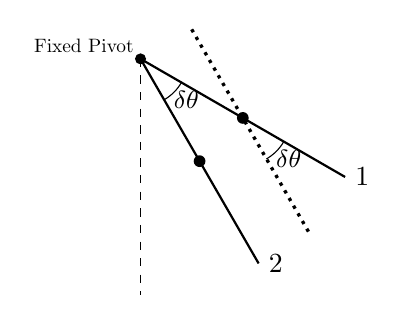
\begin{tikzpicture}[>=stealth]
  \fill (0, 0) circle (2pt) node[above left, scale=0.7] {Fixed Pivot};
  \draw[dashed]  (0, 0) -- (0, -3);
  \draw[rotate=30, thick] (0, 0) -- (0, -3) node[midway, fill=black, circle, inner sep=1.5pt] {} node[right] {2};
  \draw[rotate=30, dotted, xshift=0.75cm, very thick] (0, 0) -- (0, -3);
  \draw[rotate=60, thick] (0, 0) -- (0, -3) node[midway, fill=black, circle, inner sep=1.5pt] {} node[right] {1};
  \draw[rotate=30] (0, -0.6) arc [start angle=-90,end angle=-60,radius=0.6] node[pos=0, right] {\small$\delta\theta$};
  \draw[rotate=30] (0.75, -1.9) arc [start angle=-90,end angle=-60,radius=0.6] node[pos=0, right] {\small$\delta\theta$};
\end{tikzpicture}
\end{center}
We see that the change in the angle $\theta$ at the pivot between positions 1 and 2 is the same as the change in the angle of the rod about the centre of mass and so the rate of change of both angles is equal.

More generally, the angular velocity is the same about any point on the body and so we can use $\dot{\theta}$ as angular velocity, even though $\theta$ is about a different point.

Using \cref{rigidKESplit}, we have:
\[
  T = \frac{1}{2} M v^{2}_{\text{CoM}} + \frac{1}{2} I_{\text{CoM}}\dot{\theta}^2 \\
\]
Since the axis through the pivot and the axis through the CoM are parallel, we can parallel axis theorem (\cref{parallelAxisTheorem}) and so:
\[
  I = I_{\text{CoM}} + M\left(\frac{L}{2}\right)^2
\]
Subsisting back in along with $v_{\text{CoM}}$ yields:
\begin{align*}
  T &= \frac{1}{2} M \left(\frac{L^2}{4}\right) \dot{\theta}^2 + \frac{1}{2}[I - M(L/2)^2]\dot{\theta}^2 \\
    &= \frac{1}{2} I \dot{\theta}^2
\end{align*}
which agrees with the first method.

\subsubsection{Finding the Equation of Motion}
Since we have the kinetic energy $T$, we just need the potential $V$.
\begin{center}
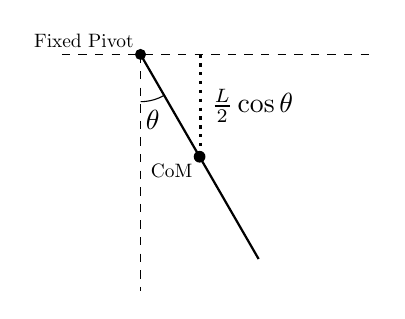
\begin{tikzpicture}[>=stealth]
  \fill (0, 0) circle (2pt) node[above left, scale=0.7] {Fixed Pivot};
  \draw[dashed]  (0, 0) -- (0, -3);
  \draw[dashed] (-1, 0) -- (3, 0);
  \draw[rotate=30, thick] (0, 0) -- (0, -3) node[midway, below left, scale=0.7] {CoM} node[midway, fill=black, circle, inner sep=1.5pt] {};
  \draw (0, -0.6) arc [start angle=-90,end angle=-60,radius=0.6] node[midway, below] {$\theta$};
  \draw[dotted, very thick] (0.76, 0) -- (0.76, -1.3) node[midway, right] {$\frac{L}{2} \cos \theta$};
\end{tikzpicture}
\end{center}
Using \cref{rigidPotential} with $R_z(t) = -\frac{L}{2} \cos \theta(t)$:
\[
  V = -Mg \left(\frac{L}{2} \cos \theta\right)
\]
Note that we need the minus sign so that as $\theta$ increases, the potential energy increases (i.e. becomes less negative).

The total energy $E$ is then:
\[
  E = \frac{1}{2}I \dot{\theta}^2 - Mg \frac{L}{2} \cos \theta
\]
The energy is conserved and so we impose that $\deriv{E}{t} = 0$:
\[
  \deriv{E}{t} = \frac{1}{2} I \cdot 2 \dot{\theta} \ddot{\theta} + Mg \frac{L}{2} \dot{\theta} \sin \theta = 0
\]
If we assume that the pendulum is not constantly at rest (i.e. $\dot{\theta}$ is not identically 0) then:
\[
  I \ddot{\theta} = - Mg \frac{L}{2} \sin \theta
\]
Again, this is like a rotational equation of motion using $I$ like the ``rotational mass''.
\subsection{Slipping and Rolling}
One type of motion that we have seen before is \textit{frictionless sliding}.
This is when there is translational motion but no rotational motion.

Another type of motion is \textit{no-slip rolling}.
This is when there is rotational motion with the additional requirement that $v = a \dot{\theta}$ and occurs when the friction between the ball and the ground is is so strong that the point of contact between the ball and the ground has zero velocity between the ground at the instant of contact.
\begin{center}
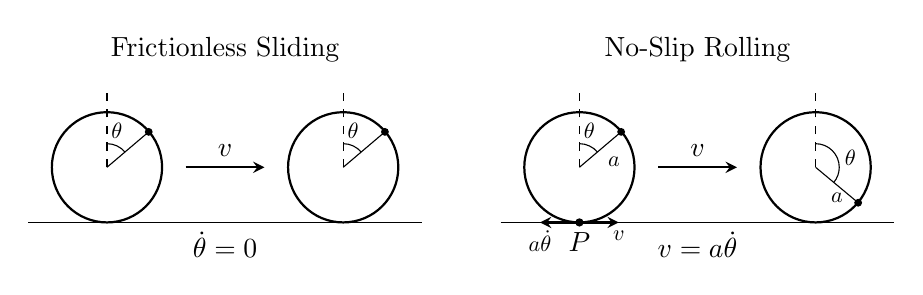
\begin{tikzpicture}[>=stealth]
  \node at (2.5, 2.2) {Frictionless Sliding};
  \draw (0, 0) -- (5, 0);
  \draw[thick] (1, 0.7) circle (0.7);
  \draw[thick] (4, 0.7) circle (0.7);
  \draw (1, 1) arc [start angle=90,end angle=40,radius=0.3] node[midway, above, scale=0.8] {$\theta$};
  \draw[dashed] (1, 0.7) -- (1, 1.7);
  \draw (1, 0.7) -- (1.53, 1.15) node[pos=1, fill=black, circle, inner sep=1pt] {};
  \begin{scope}[xshift=3cm]
    \draw (1, 1) arc [start angle=90,end angle=40,radius=0.3] node[midway, above, scale=0.8] {$\theta$};
    \draw[dashed] (1, 0.7) -- (1, 1.7);
    \draw (1, 0.7) -- (1.53, 1.15) node[pos=1, fill=black, circle, inner sep=1pt] {};
  \end{scope}
  \draw[->, thick] (2, 0.7) -- (3, 0.7) node[midway, above] {$v$};
  \node[below] at (2.5, 0) {$\dot{\theta} = 0$};

  \begin{scope}[xshift=6cm]
    \node at (2.5, 2.2) {No-Slip Rolling};
    \draw (0, 0) -- (5, 0);
    \draw[thick] (1, 0.7) circle (0.7);
    \draw[thick] (4, 0.7) circle (0.7);
    \draw (1, 1) arc [start angle=90,end angle=40,radius=0.3] node[midway, above, scale=0.8] {$\theta$};
    \draw[dashed] (1, 0.7) -- (1, 1.7);
    \draw (1, 0.7) -- (1.53, 1.15) node[midway, below right, scale=0.8] {$a$} node[pos=1, fill=black, circle, inner sep=1pt] {};

    \fill (1, 0) circle (1.5pt);
    \node[below] at (1, 0) {$P$};
    \draw[thick, ->] (1, 0) -- (0.5, 0) node[below, scale=0.8] {$a \dot{\theta}$};
    \draw[thick, ->] (1, 0) -- (1.5, 0) node[below, scale=0.8] {$v$};
    \begin{scope}[xshift=3cm]
      \draw (1, 1) arc [start angle=90,end angle=-40,radius=0.3] node[midway, right, scale=0.8] {$\theta$};
      \draw[dashed] (1, 0.7) -- (1, 1.7);
      \draw (1, 0.7) -- (1.54, 0.25) node[midway, below, scale=0.8] {$a$} node[pos=1, fill=black, circle, inner sep=1pt] {};
    \end{scope}
    \draw[->, thick] (2, 0.7) -- (3, 0.7) node[midway, above] {$v$};
    \node[below] at (2.5, 0) {$v = a \dot{\theta}$};
  \end{scope}
\end{tikzpicture}
\end{center}
If we consider the point point of contact $P$, it has velocity $v$ to the right from the translational motion of the rigid body (it is being pulled along since distances between particles must remain constant), but also has velocity $a \dot{\theta}$ to the left from the rotational motion of the rigid body.
Since we have imposed the restriction that $v = a \dot{\theta}$, $P$ has no velocity relative to the ground at the instant it contacts the ground.

In the case of non-slip rolling, The kinetic energy is:
\begin{align*}
  T &= \frac{1}{2} M v^2 + \frac{1}{2}I\omega^2 \\
    &= \frac{1}{2} \left(M + \frac{I}{a^2}\right)v^2 \text{ as $\omega = \dot{\theta} = \frac{v}{a}$}
\end{align*}
We can interpret this as rolling increasing the ``effective mass'' of the ball.

Friction is needed for this kind of motion to happen, however, because there is no relative velocity between the point of contact and the ground, no work is done by the friction force and thus energy is conserved when a body is no-slip rolling.
The only role of friction here is to impose the no-slip condition.

To check that energy is conserved when rolling when a frictional force $f$ acts at the contact point, we can differentiate the kinetic energy:
\[
  E = \frac{1}{2}M \dot{x}^2 + \frac{1}{2} I \dot{\theta}^2 \implies \deriv{E}{T} = M \dot{x}\ddot{x} + I \dot{\theta}\ddot{\theta}
\]
Recall from \cref{torqueMomentOfInertia} that the torque is $G = I \dot{\omega} = I \ddot{\theta}$.
Since the frictional force $f$ is acting at a perpendicular distance $a$, the torque $G = af$ and so $I \ddot{\theta} = af$.
Furthermore, using Newton's equation $M\ddot{x}$ is the force $f$ acting on the ball and so:
\begin{align*}
  \deriv{E}{t} &= \dot{x}(-f) + \dot{\theta}af \\
               &= f(-\dot{x} + a \dot{\theta}) \text{ as rolling: $\dot{x} = v = a \dot{\theta}$} \\
               &= 0
\end{align*}
So the energy is conserved, despite the presence of a frictional force.
\begin{example}[Ball Rolling on a Slope]
  Consider a ball \textbf{no-slip rolling} down a slope that makes an angle $\alpha$ with the horizontal:
  \begin{center}
  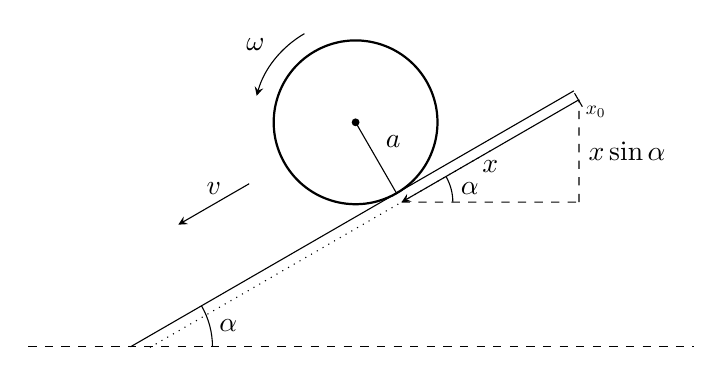
\begin{tikzpicture}[>=stealth, scale=1.3]
    \draw[dashed] (-1, 0) -- (5.5, 0);
    \draw (0.8, 0) arc [start angle=0,end angle=30,radius=0.8] node[midway, right] {$\alpha$};
    \draw[rotate=30, thick] (3, 0.8) circle (0.8);
    \draw[rotate=30] (3, 0.8) node[fill=black, circle, inner sep=1pt] {} -- (3, 0) node[midway, above right] {$a$};
    \draw[rotate=30, ->] (3, 0.8) ++ (90:1) arc (90:135:1) node[midway, above left] {$\omega$};
    \draw[rotate=30] (0, 0) -- (5, 0);
    \draw[rotate=30, ->] (1.8, 0.8) -- (1, 0.8) node[midway, above] {$v$};
    \draw[rotate=30, |->] (5, -0.1) node[below right, scale=0.7] {$x_0$} -- (3, -0.1) node[midway, below] {$x$};
    \draw[rotate=30, dotted] (4, -0.1) -- (0.15, -0.1);
    \draw[rotate=30, dashed]  (3, -0.1) -- (4.5, -0.966);
    \draw[rotate=30, dashed] (4.5, -0.966) -- (5, -0.1) node[midway, right] {$x \sin \alpha$};
    \draw[rotate=30] (3, -0.1) ++ (0:0.5) arc (0:-30:0.5) node[midway, right] {$\alpha$};
  \end{tikzpicture}
  \end{center}
  We know the kinetic energy so just need the potential energy.
  Using \cref{rigidPotential} with $R_z(t) = -x(t)\sin\alpha$:
  \[
    V = -Mgx\sin\alpha
  \]
  It is irrelevant that we did not measure from the CoM as the difference would be just a constant offset that would disappear during differentiation.

  Thus the conserved energy is:
  \[
    E = \frac{1}{2} \left(M + \frac{I}{a^2}\right) \dot{x}^2 - Mgx\sin\alpha
  \]
  Since $\deriv{E}{t} = 0$, the equation of motion is:
  \[
    \left(M + \frac{I}{a^2}\right) \ddot{x} = Mg\sin\alpha
  \]
\end{example}
\section{Normal Forces and Dry Friction}
\label{dryFriction}
\subsection{Normal Forces}
Objects do not fall through each other because they exert a \textit{normal force} on each other.
Similarly to friction, this is not a fundamental force, but is a manifestation of various microscopic forces between molecules, however, in Newtonian mechanics, we model the overall effect as force normal to the contact surface between the objects.

For example, the block has a downward force of magnitude $mg$ acting on it due to gravity and so the block exerts a normal force of magnitude $mg$ on the table.
The table then exerts a normal force of the same magnitude but in the opposite direction:
\begin{center}
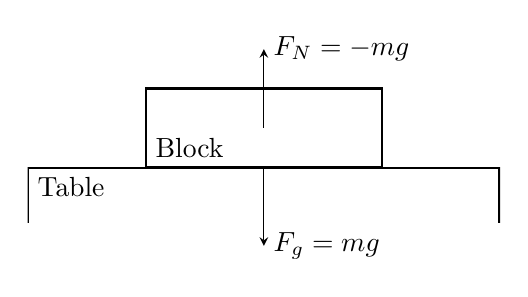
\begin{tikzpicture}[>=stealth]
  \begin{scope}
    \clip (-3 , -0.7) rectangle (3, 0);
    \draw[very thick] (-3, -1) rectangle (3, 0);
  \end{scope}
  \draw[thick] (-1.5, 0) rectangle (1.5, 1);
  \draw[->] (0, 0.5) -- (0, 1.5) node[right] {$F_N = -mg$};
  \draw[->] (0, 0) -- (0, -1) node[right] {$F_g = mg$};
  \node[below left] at (-1.9, 0) {Table};
  \node[above right] at (-1.5, 0) {Block};
\end{tikzpicture}
\end{center}
On a slope, we have to resolve the gravitational force on the block into two components as the normal force only acts normal to the surface:
\begin{center}
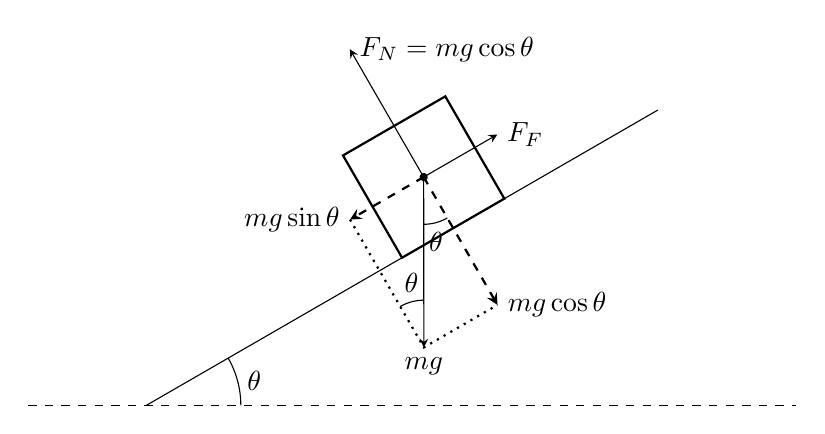
\begin{tikzpicture}[>=stealth, scale=1.5]
  \draw[dashed] (-1, 0) -- (5.5, 0);
  \draw (0, 0) ++ (0:0.8) arc (0:30:0.8) node[midway, right] {$\theta$};
  \draw[rotate=30] (3, 0.5) ++ (-90:0.4) arc (-90:-120:0.4) node[midway, below] {$\theta$};
  \draw[rotate=30] (2.28, -0.75) ++ (90:0.4) arc (90:60:0.4) node[midway, above] {$\theta$};
  \draw[rotate=30, thick] (2.5, 0) rectangle (3.5, 1);
  \fill[rotate=30] (3, 0.5) circle (1pt);
  \draw[rotate=30, ->, dashed, thick] (3, 0.5) -- (3, -0.75) node[right] {$mg \cos \theta$};
  \draw[rotate=30, ->] (3, 0.5) -- (3, 1.75) node[right] {$F_N = mg\cos\theta$};
  \draw[rotate=30, ->, dashed, thick] (3, 0.5) -- (2.28, 0.5) node[left] {$mg\sin\theta$};
  \draw[rotate=30, ->] (3, 0.5) -- (2.28, -0.75) node[below] {$mg$};
  \draw[rotate=30, dotted, thick] (2.28, 0.5) -- (2.28, -0.75) -- (3, -0.75);
  \draw[rotate=30, ->] (3, 0.5) -- (3.72, 0.5) node[right] {$F_F$};
  \draw[rotate=30] (0, 0) -- (5, 0);
\end{tikzpicture}
\end{center}
The normal force does not prevent the object from sliding down the slope, this is instead due to the \textit{dry friction force}, $F_F$.
Similarly to fluid drag from \cref{frictionDrag}, dry friction always acts to oppose motion, however, dry friction is independent of speed.

The frictional force takes the minimal value required to stop the object from moving but is limited by:
\[
  F_{F} \leq \mu F_N
\]
where $\mu$ is the \textit{coefficient of friction} which is typically close to, but less than 1.
If the object is at the \textit{point of slipping} or has started to move then $F_F$ takes its maximal value:
\[
  F_{F} = \mu F_n
\]
\subsection{Elastic Bounces}
Normal forces also produce \textit{elastic bounces}.
\begin{definition}[Elastic Collision]
  An \textit{elastic collision} is a collision in which energy is conserved.
\end{definition}
Consider a ball with incoming momentum $\vec{p}$ that bounces off a wall elastically resulting in an outgoing momentum $\vec{q}$:
\begin{center}
\begin{tikzpicture}[>=stealth, decoration={
      markings,
      mark=at position 0.3 with {\arrow{>}},
      mark=at position 0.6 with {\arrow{>}},
      mark=at position 0.9 with {\arrow{>}}
    }
  ]
  \draw[thick] (-3, -0.5) -- (3, -0.5);
  \draw (0, 0) circle (0.5);
  \draw[dashed] (-3, 0) -- (3, 0);
  \draw (0, 0) ++ (0:1) arc (0:30:1) node[midway, right] {$\beta$};
  \draw (0, 0) ++ (150:1) arc (150:180:1) node[midway, left] {$\alpha$};
  \draw[rotate=30] (2.5, 0) circle (0.5);
  \draw[rotate=30, postaction={decorate}] (0, 0) -- (2.5, 0) node[midway, above left] {$\vec{q}$};

  \draw[rotate=150] (2.5, 0) circle (0.5);
  \draw[rotate=150, postaction={decorate}] (2.5, 0) -- (0, 0) node[midway, above right] {$\vec{p}$};

  \draw[->] (0, 0) -- (0, 1) node[above] {$F_N$};
  \begin{scope}[xshift=3.4cm]
    \draw[->] (-0.1, 0)  -- (1, 0) node[right] {$x$};
    \draw[->] (0, -0.1)  -- (0, 1) node[above] {$y$};
  \end{scope}
  \node[below right] at (-3, -0.5) {Wall};
\end{tikzpicture}
\end{center}
The normal force on impact is in the direction normal to the surface at the point of impact, i.e. in the $y$ direction above

The total momentum is conserved and so the total momentum of the wall and the wall before the collision must be same the same as afterwards.
There is no external force acting on the ball in $x$ direction so the component velocity in the $x$ direction is unchanged and so we consider only the $y$ component of the momentum.

Assuming that the wall is stationary before the collision, we have:
\[
  p_y = q_y + Q_y
\]
where $Q_y$ is the momentum of the wall after the collision.

Since we know velocity in the $x$ direction is conserved, we only need to worry about energy being conserved in the $y$ direction:
\[
  \frac{p^2_y}{2m} = \frac{q^2_y}{2m} + \frac{Q^2_y}{2M}
\]
where $m$ is the mass of the ball and $M$ is the mass of the wall.
Substituting $p_y$ in, we see that:
\[
  \frac{1}{2m}(\cancel{q^2_y} + Q^2_y + 2Q_y q_y) = \cancel{\frac{q^2_y}{2m}} + \frac{Q^2_y}{2M}
\]
Since, $M \gg m$, we have that $\frac{Q^2_y}{2M} \ll \frac{Q^2_y}{2m}$ so $\frac{Q^2_y}{2M}$ is negligible and can be ignored.
Therefore:
\[
  \frac{1}{2m}(Q^2_y + 2Q_yq_y) = 0 \implies Q_y = -2q_y
\]
so $p_y = q_y - 2q_y = -q_y$.
That is, the $y$ component of the momentum is flipped by the collision and so $\alpha = \beta$.

This change in momentum $\Delta p$ of the ball over a short time is called an \textit{impulse} $I$.
\end{document}
